\documentclass[pdf]{article}
\usepackage{pgfplots} 
\usepgfplotslibrary{external} 
\tikzexternalize 
\usepackage{tikz} 
\usepackage{amsmath} 
\usetikzlibrary{calc} 
\pgfplotsset{compat = newest, every axis plot post/.style={line join=round},every non boxed x axis/.append style={x axis line style=-}, every non boxed y axis/.append style={y axis line style=-}}
\begin{document} 
	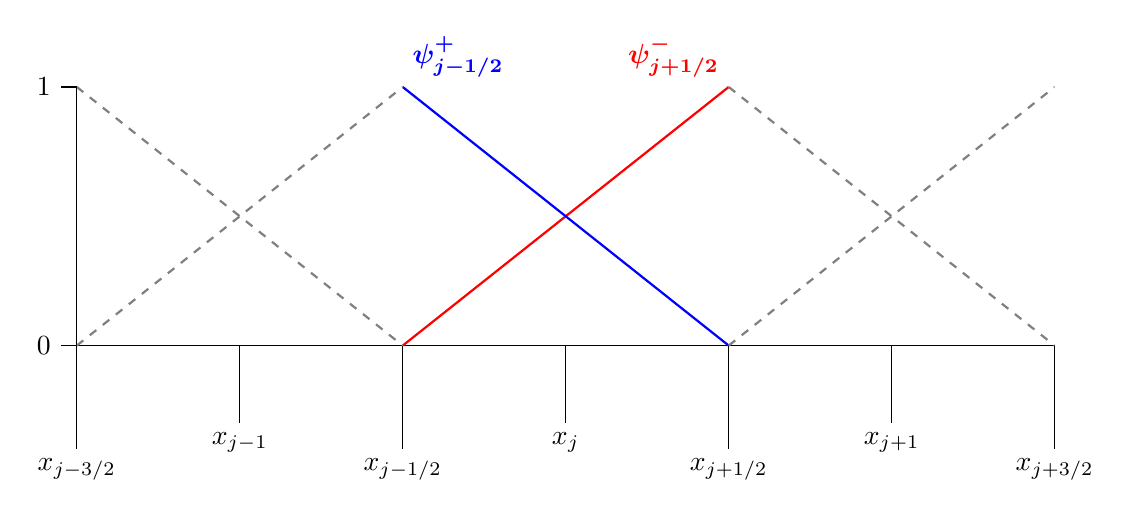
\begin{tikzpicture} 
	\begin{axis}[ 
	width = 14cm,
	height = 7cm,
	axis lines=left, 
	xticklabels=\empty,
	x axis line style={draw=none},
	y axis line style={draw=none},
	ytick=\empty,
	xtick = \empty,
	clip mode=individual,
	xmin=0, 
	xmax=3, 
	ymin = -.45, 
	ymax = 1.2]
		
		\draw (axis cs:3,0) -- (axis cs:0,0);
		\draw (axis cs:0,1) -- (axis cs:0,0);
		
		\draw[thin] (axis cs:0,0) -- (axis cs:0,-0.4);
		\draw[thin] (axis cs:0.5,0) -- (axis cs:0.5,-0.3);
		
		\draw[thin] (axis cs:1,0) -- (axis cs:1,-0.4);
		\draw[thin] (axis cs:1.5,0) -- (axis cs:1.5,-0.3);
		\draw[thin] (axis cs:2,0) -- (axis cs:2,-0.4);

		\draw[thin] (axis cs:2.5,0) -- (axis cs:2.5,-0.3);
		\draw[thin] (axis cs:3,0) -- (axis cs:3,-0.4);
		
		\draw[thin] (axis cs:0,1) -- (axis cs:-0.05,1);
		\draw[thin] (axis cs:0,0) -- (axis cs:-0.05,0);
		
		\node[left] at (-0.05,0) {$0$};
		
		\node[left] at (-0.05,1) {$1$};
		
		\node[below] at (0,-0.4) {$x_{j-3/2}$};
		\node[below] at (0.5,-0.3) {$x_{j-1}$};
		
		\node[below] at (1,-0.4) {$x_{j-1/2}$};
		\node[below] at (1.5,-0.3) {$x_{j}$};
		\node[below] at (2,-0.4) {$x_{j+1/2}$};
		
		\node[below] at (2.5,-0.3) {$x_{j+1}$};
		\node[below] at (3,-0.4) {$x_{j+3/2}$};
		
	\addplot [smooth, thick, red] coordinates { (1,0)  (2,1)};
	\addplot [smooth, thick, blue] coordinates { (1,1)  (2,0)};
	
	\addplot [dashed, thick,gray] coordinates { (0,0)  (1,1)};
	\addplot [dashed, thick,gray] coordinates { (0,1)  (1,0)};
	
	\addplot [dashed, thick,gray] coordinates { (2,0)  (3,1)};
	\addplot [dashed, thick,gray] coordinates { (2,1)  (3,0)};
	
	
	\node[above right] at (1,1) {\color{blue}$\boldsymbol{\psi^+_{j-1/2}}$};
	\node[above left] at (2,1) {\color{red}$\boldsymbol{\psi^-_{j+1/2}}$};
	
			
		
	\end{axis} 
	\end{tikzpicture} 
\end{document}